\documentclass[12pt, twocolumn]{report}
\usepackage{amsfonts}
\usepackage{amsmath}
\usepackage{amssymb}
\usepackage{caption}
\usepackage{subcaption}
\usepackage{setspace}
\usepackage{geometry}
\usepackage{hyperref}
\usepackage{graphicx}

\onehalfspacing
\geometry{margin=25mm}

\author{Liuchuyao Xu}
\title{General-purpose Computing on Graphics Processing Units for Real-time Analysis of Scanning Electron Microscope Images}

\begin{document}
\maketitle

\begin{abstract}
\end{abstract}

\chapter{Introduction}
\paragraph{}
The scanning electron microscope (SEM) is a type of microscope that produces images using signals generated from the interaction between electrons and the surface under observation. It has higher resolutions than traditional optical microscopes---an SEM can have a resolution lower than one nanometre, whereas that of an optical microscope is limited to a few hundred nanometres. This has benefited a variety of fields by allowing scientists to see micro-details of objects that were previously impossible to observe. For example, the SEM can be used to study structures of semiconductor devices \cite{SEM for semiconductors} and to view changes in bacterial cells \cite{SEM for baterial cells}.

\paragraph{}
Fig. \ref{SEM basic construction} illustrates how an SEM works. The electron gun generates an electron beam, which is transformed into an electron probe after passing through the condenser lens and objective lens. It is then scanned across the specimen under the effect of the scanning coil. As a result of the interaction between the incident electrons and the specimen, some electrons (which are called secondary electrons) are emitted from the specimen. The detector collects the secondary electrons and generates signals based on their energy levels. The display unit uses the signals to produce one image after each complete scan of the specimen.

\begin{figure}[htbp]
    \centering
    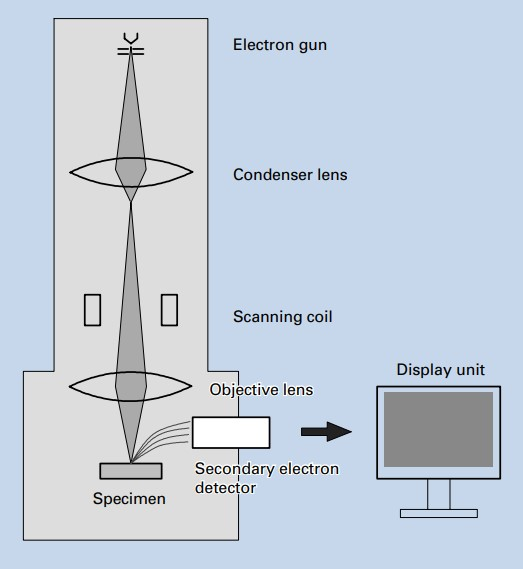
\includegraphics[width=0.45\textwidth]{Figures/SEM basic construction.jpg}
    \caption{Basic construction of an SEM \cite{SEM A to Z}.}
    \label{SEM basic construction}
\end{figure}

\paragraph{}
Many image analysis methods have applications in the field of SEM, and the fast Fourier transform is an especially popular one since it can be used to evaluate the focusing and astigmatism of an SEM [see section TBC]; however, due to the complexity of the algorithm and a lack of fast hardware, real-time analysis had been either impossible or impractical in the past. In 1997, with an advanced central processing unit (CPU)---the Pentium Pro, it was only possible to achieve a refresh rate of 0.6 frames per second for 8-bit 1024 $\times$ 1024 input images \cite{SEM image sharpness measurement}. Although the enhancement of CPUs has enabled faster computations throughout the years, what really brings the speed to a different level is the development of graphics processing units (GPUs).

\paragraph{}
The GPU used to be a highly specialised hardware that was designed to excel in rendering complex, high-resolution, real-time 3D scenes for games; however, its special architecture has made it outperform CPUs in many other areas and resulted in the birth of the idea of general-purpose computing on graphics processing units (GPGPU) \cite{GPU computing}, where GPUs are used to perform computations that are traditionally handled by CPUs.

\paragraph{}
A key characteristic of GPUs is massive parallelism. Depending on their positions, pixels in a 3D scene often require different processing to achieve effects such as lighting, blurring, and fogging. GPUs do this by breaking down the scene into fragments and manipulating each fragment individually. Modern GPUs have thousands of parallel processor cores each running tens of parallel threads to meet the the high requirement for parallelism. For example, the NVIDIA GeForce GTX 1060 has 1280 cores and each of them is capable of running 16 threads; a similarly prices CPU---the Intel i7-7700---has only 4 cores each running 8 threads. It is worth mentioning that the processing cores on a GPU are not as sophisticated as a full CPU and run at a lower clock frequency. The processor clock frequency of the GTX 1060 is 1708 MHz whereas the i7-7700 has a base processor frequency of 3600 MHz. This means that GPGPU is more useful for applications that involve simple, repetitive, parallel tasks. A recent example is deep learning, where computations that follow the same logical sequence of control need to be performed on a deep network of nodes. Typical deep learning networks in 2015 consist of about one million nodes \cite{Deep learning}, which means that the computations cannot be done efficiently on a CPU.

\paragraph{}
This report investigates the gain in calculation speeds from the use of GPUs, and presents a diagnostic tool developed based on GPGPU, which can perform real-time histogram equalisation and FFT on images captured by an SEM. The tool was used to implement an automatic focusing and astigmatism correction algorithm, and the results are discussed.

\chapter{The gain in calculation speeds from the use of GPUs}
\section{GPU computing}
\paragraph{}
The GPU is designed to meet the high demand in parallelism for fast rendering of scenes on displays. For example, a 1080p display refreshing at 60 Hz requires $60 \times 1920 \times 1080 = 124,416,000$ values to be computed in each second, which cannot be done efficient enough in the sequential manner used by the CPU. It describes an image using graphics primitives as shown in Fig. \ref{GPU graphics primitives}. To construct the image, the primitives are passed through the graphics pipeline of the GPU, which can be divided into the following stages:
\begin{itemize}
    \item Vertex generation. A list of vertices are generated to represent the image as a 3D triangle mesh, as illustrated by Fig. \ref{GPU graphics triangle mesh}.
    \item Triangle generation. The vertices are assembled into triangles, which are the fundamental hardware-supported primitive in modern GPUs.
    \item Fragment generation. The triangles are mapped to blocks of pixels on the screen; each block is called a ``fragment''.
    \item Fragment processing. The fragments are shaded based on colour and texture information to determine their final colour.
    \item Composition. A final image is created by assembling the fragments.
\end{itemize}
The processing of primitives within each stage follow the same logical sequence of control, but the data are different. This pattern is called ``single instruction multiple data'' (SIMD). The GPU has a large array of SIMD, multi-threaded processing cores sharing the same global memory, and it divides the cores among the stages such that the pipeline is divided in \textit{space}, not time. Each primitive is processed by a thread of one of the processors.

\begin{figure}[htbp]
    \centering
    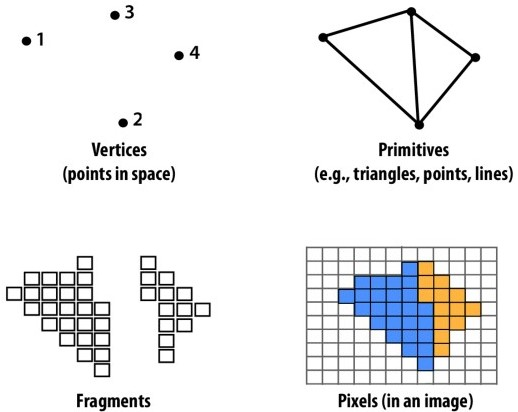
\includegraphics[width=0.45\textwidth]{Figures/GPU graphics primitives.jpg}
    \caption{Graphics primitives \cite{GPU architecture lecture}.}
    \label{GPU graphics primitives}
\end{figure}

\begin{figure}[htbp]
    \centering
    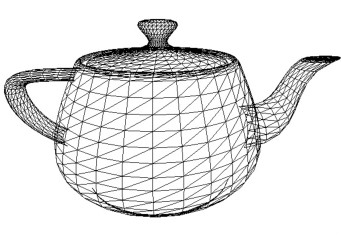
\includegraphics[width=0.45\textwidth]{Figures/GPU graphics triangle mesh.jpg}
    \caption{Representing an image as a 3D triangle mesh \cite{GPU architecture lecture}.}
    \label{GPU graphics triangle mesh}
\end{figure}

The parallel structure of the GPU can also provide a significant speed improvement in general-purpose computing. Take the addition of two vectors of size $N$ as an example:
\begin{equation*}
    \boldsymbol{v_3} = \boldsymbol{v_1} + \boldsymbol{v_2}
\end{equation*}
The CPU divides the task in time and does:
\begin{align*}
    & \text{Time 1: } \boldsymbol{v_3}[0] = \boldsymbol{v_1}[0] + \boldsymbol{v_2}[0] \\
    & \vdots \\
    & \text{Time n: } \boldsymbol{v_3}[n] = \boldsymbol{v_1}[n] + \boldsymbol{v_2}[n] \\
\end{align*}
This results in a time complexity of $O(N)$. The GPU achieves a time complexity of $O(1)$ by dividing the task in space, i.e. among threads, and does:
\begin{align*}
    & \text{Time 1: }
\begin{cases}
    & \text{Thread 1: } \boldsymbol{v_3}[0] = \boldsymbol{v_1}[0] + \boldsymbol{v_2}[0] \\
    & \vdots \\
    & \text{Thread n: } \boldsymbol{v_3}[n] = \boldsymbol{v_1}[n] + \boldsymbol{v_2}[n] \\
\end{cases}
\end{align*}
The task is an SIMD task---the program takes one element from each of the vectors and perform addition on them, but the data handled by each thread is different, it can therefore make full use of the SIMD cores of the GPU. When $N$ is small, the overhead in allocating the resources means that the speed improvement is negligible; however, as $N$ grows large, the reduction in time complexity quickly compensates for the overhead and makes the GPU much faster than the CPU.

\paragraph{}
Prior to 2007, to use GPUs for general-purpose computing, the user must write programs using the graphics application programming interface (API) since it was the only interface to GPU hardware. The programming model can be summarised as below:
\begin{itemize}
    \item The user specifies geometry that covers a region on the screen.
    \item The user sets parameters of the pipeline (e.g., ``lighting'' and ``texture'' information).
    \item The user provides the fragment processing program (kernel).
    \item The GPU produces an output ``image'' and stores it in global memory.
\end{itemize}
This was a major problem in GPGPU because many general-purpose tasks have nothing to do with graphics and are difficult to implement using the graphics API. 

\paragraph{}
The introduction of CUDA changed the situation by providing a more natural, direct, non-graphics interface. The new programming model can be summarised as below:
\begin{itemize}
    \item The user defines the computation as a structured grid of threads.
    \item The GPU executes each thread and stores the results in global memory.
\end{itemize}
This model allows the user to directly define threads that are run on the processing cores of the GPU, eliminating the complexity in translating the program into graphics pipeline language, which makes it easier for the user to take full advantage of the GPU's power. The following section describes an experiment conducted to determine the gain in calculation speeds from using CUDA.

\section{Experiment, results and discussions}


\chapter{Conclusions}

\begin{thebibliography}{00}
    \bibitem{SEM for semiconductors}
    C. REEVES, ``The uses of scanning electron microscopy for studying semiconductor devices,'' International Journal of Electronics, vol. 77, no. 6, pp. 919-928, 1994, doi: 10.1080/00207219408926111.

    \bibitem{SEM for baterial cells}
    T. Cushnie, N. O’Driscoll and A. Lamb, ``Morphological and ultrastructural changes in bacterial cells as an indicator of antibacterial mechanism of action,'' Cellular and Molecular Life Sciences, vol. 73, no. 23, pp. 4471-4492, 2016, doi: 10.1007/s00018-016-2302-2.

    \bibitem{SEM A to Z}
    ``SEM A to Z,'' Jeol.co.jp, [Online], available: \url{https://www.jeol.co.jp/en/applications/pdf/sm/sem_atoz_all.pdf}. [Accessed: 18 May 2020].

    \bibitem{SEM image sharpness measurement}
    A. Vladár, M. Postek and M. Davidson, ``Image sharpness measurement in scanning electron microscopy-part II,'' Scanning, vol. 20, no. 1, pp. 24-34, 2006, doi: 10.1002/sca.1998.4950200104.

    \bibitem{GPU computing}
    J. D. Owens, M. Houston, D. Luebke, S. Green, J. E. Stone and J. C. Phillips, ``GPU Computing,'' in Proceedings of the IEEE, vol. 96, no. 5, pp. 879-899, May 2008, doi: 10.1109/JPROC.2008.917757.

    \bibitem{Deep learning}
    Ian Goodfellow; Yoshua Bengio; Aaron Courville, ``Deep learning,'' in Deep Learning, The MIT Press, 2017, p. 23.

    \bibitem{GPU architecture lecture}
    ``GPU Architecture and CUDA Programming,'' Carnegie Mellon University, 2017, [Online], available: \url{http://15418.courses.cs.cmu.edu/spring2017/home}. [Accessed: 19 May 2020].
\end{thebibliography}
\end{document}
